% id: 17-15
% book: 개념원리 기하 · 01 포물선의 방정식
% section: 필수·발전 예제
% figure: crop:fig-17-15.png
% answer: $3$
% answer_source: 답지
% variant_level: 0 (원본 전사)
% 이 파일은 build.mjs 가 items.json 에서 만든다. 고칠 때는 items.json 을 고친다.
\smash{\raisebox{1.5mm}{\dmkichul{개념원리 기하 17쪽 15번 · 확인체크}}}
\noindent\begin{minipage}[t]{0.58\linewidth}\vspace{0pt}\raggedright 오른쪽 그림과 같이 포물선 $x^2=4y$의 초점~$\pt{F}$를 지나는 직선이 포물선과 만나는 두 점을 각각 $\pt{A}$, $\pt{B}$라 하고, 두 점~$\pt{A}$, $\pt{B}$에서 $x$축에 내린 수선의 발을 각각 $\pt{C}$, $\pt{D}$라 하자. $\seg{AB}=5$일 때, $\seg{AC}+\seg{BD}$의 값을 구하시오.\end{minipage}\hfill\begin{minipage}[t]{0.4\linewidth}\vspace{0pt}\centering \setlength{\dmfigw}{102.8pt}\ifdim\dmfigw>\linewidth\setlength{\dmfigw}{\linewidth}\fi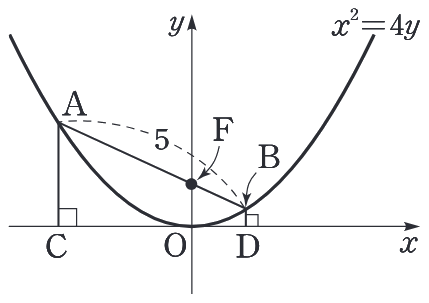
\includegraphics[width=\dmfigw]{figures/fig-17-15.png}\end{minipage}\par
